\documentclass{memoria}


\begin{document}

\portada{Informe Entrega 2: Diseño Arquitectural}{Gerson Aguirre Pavez\\Max Chacón Villanueva\\Daniel Gacitúa Vásquez\\Elías González Marincovic\\Nicolás Rozas Sepúlveda}{\textbf{Profesores:}\\Mauricio Marín Caihuán\\Rodrigo Vásquez Fernández\\\textbf{Ayudante:\\}José Orellana}{\today}


\indices

\capitulonn{INTRODUCCIÓN.}

En esta entrega se presenta la etapa de diseño arquitectural de la aplicación \textbf{\textsl{BitPhoto}}, réplica de \textsl{Flickr}.  El objetivo de esta etapa es construir la arquitectura básica para el funcionamiento de la aplicación, definiendo los diversos componentes del sistema acordes a la solución necesitada. Para especificar de manera más detallada la arquitectura del sistema se utilizará el modelo 4 + 1 vistas, el cual nos permite definir en cada una de sus vistas una parte esencial de la arquitectura del sistema, y de manera conjunta ofrecer una visión específica en diversos niveles, desde saber cuáles son los componentes involucrados, dónde se despliegan, y de qué manera interactúan entre ellos para cumplir con los requerimientos especificados en la entrega anterior, correspondiente a la ingeniería de requerimientos.
 
En este informe se presenta inicialmente un marco teórico utilizado para contextualizar el contenido y al mismo tiempo hacer referencia conceptual a éste. Luego continuando con el cumplimiento de los objetivos, se presenta el modelo 4 + 1 vistas, que servirá para explicar todos los elementos anteriormente mencionados. Para desarrollar este modelo, en primera instancia se trata la \textsl{Vista Lógica}, y es en esta parte donde se detallan los módulos del sistema que entregan la funcionalidad característica del mismo, asemejándose al diagrama de clases presentado con anterioridad. Continuando con las vistas, se presenta la \textsl{Vista de Proceso} donde se muestran los aspectos de concurrencia y sincronización correcta del sistema para el óptimo funcionamiento de la aplicación. Luego, la \textsl{Vista Física} permite observar el \textsl{mapeo} del software y analizar de qué manera se distribuye y posteriormente, en la \textsl{Vista de Desarrollo} se muestra la forma en que se despliega el software en el ambiente de desarrollo. 

Después de las vistas, se presentan eventuales escenarios, en los cuales se aprecia la forma en que se comporta el sistema y de qué manera interactúan los módulos y componentes de éste para realizar determinadas acciones asociadas a los diferentes casos de uso. Luego, para dar una visión globalizada de la arquitectura del sistema, se utiliza el \textsl{framework} conceptual de \textsl{SunTone}, que se representa en forma de cubo, detallando de esta forma la calidad del sistema, los niveles de lógica y de servicios de infraestructura en cada una de sus caras. Además, con el fin de comprender de mejor manera la arquitectura del sistema, se señalan los diferentes tipos de \textsl{frameworks} tecnológicos y conceptuales utilizados, definiendo los patrones de diseños que se usarán y los problemas que estos solucionan. Por último, luego de haber especificado el diseño arquitectural, se presenta en detalle cuáles serán las tecnologías utilizadas por el sistema, describiendo cada una de éstas, señalando la versiones que se utilizarán y definiendo cuál es el problema que resuelven o la funcionalidad que aportan. 

Para finalizar el informe, se entregará un detalle sobre la planificación y organización de este \textsl{sprint}, detallando las tareas definidas y la estimación de tiempo para cada una de éstas, para luego mostrar los gráficos \textsl{Burn Down} y \textsl{Burn Up}, los que señalarán de qué manera se desarrolló el trabajo entregado con el paso de los días para hacer el análisis pertinente referente al desarrollo de la entrega, identificando las principales dificultades y los cambios realizados con respecto al \textsl{sprint} anterior, entre otras cosas. 

En resumen, se puede establecer que el objetivo de este informe es definir la arquitectura del sistema, identificando cuales deben ser los componentes del mismo, con el fin de satisfacer los requisitos especificados en la entrega pasada. También se busca definir de qué manera se distribuirán estos componentes en el sistema y en qué máquinas de hardware se van a desplegar y todo este conocimiento deberá servir como base para el desarrollo de la siguiente entrega (correspondiente al diseño detallado) donde se especificará la arquitectura pero llevada a la tecnología utilizada (especificada en este documento) y a las características propias de éstas.

%-------------------------------------------------------------------------------------
\capitulo{MARCO TEÓRICO.}

\seccion{MODELO 4+1 VISTAS.}

Este modelo, es una forma de representar una arquitectura de aplicación, el que requiere múltiples vistas para su entendimiento. Este recurso permite abordar los intereses de los distintos \textsl{stakeholders} de la arquitectura por separado: usuarios finales, desarrolladores, ingenieros de sistemas, administradores de proyecto, etc. Y de esta manera poder manejar los requisitos funcionales y no funcionales separadamente.

Las vistas definidas en este modelo, son las siguientes:

\begin{itemize}
\item \textbf{Vista Lógica}: describe el modelo de objetos del diseño cuando se utiliza un método de diseño orientado a objetos. Para modelar una aplicación que esté orientada a los datos, se puede usar un enfoque alternativo para desarrollar algún otro tipo de vista lógica, tal como diagramas de entidad-relación.
\item \textbf{Vista de Procesos}: se enfoca en la descripción de los aspectos de concurrencia y sincronización del diseño. La arquitectura de procesos toma en cuenta algunos requisitos no funcionales tales como la performance y la disponibilidad. Se centra en asuntos de concurrencia y distribución, integridad del sistema y de tolerancia a fallas. La vista de procesos también específica en cual hilo de control se ejecuta efectivamente una operación de una clase identificada en la vista lógica.
\item \textbf{Vista Física}: se encarga de describir el mapeo del software en el hardware y refleja los aspectos de distribución. La arquitectura física toma en cuenta primeramente los requisitos no funcionales del sistema tales como la disponibilidad, confiabilidad (con respecto a la tolerancia a fallas), performance (throughput), y escalabilidad. El software se ejecuta sobre una red de computadoras o sobre nodos de procesamiento (o en algunos casos tan solo nodos). Los variados elementos identificados –tales como redes, procesos, tareas y objetos– requieren ser mapeados sobre los variados nodos existentes. Se espera que se puedan utilizar diferentes configuraciones, algunas para desarrollo y pruebas, y otras para emplazar el sistema en varios sitios para distintos usuarios.
\item \textbf{Vista de Desarrollo}: escribe la organización estática del software en su ambiente de desarrollo. La vista de desarrollo se centra principalmente en la organización real de los módulos que interactúan en el sistema, en el ambiente de desarrollo del software. El software se empaqueta en partes pequeñas –como bibliotecas de programas o subsistemas– que pueden ser desarrollados por uno o un grupo pequeño de desarrolladores. Los subsistemas se organizan en una jerarquía de capas, cada una de las cuales brinda una interfaz estrecha y bien definida hacia las capas superiores.
\item \textbf{Escenarios (+1)}: corresponde a la ilustración de un conjunto reducido de casos de uso o escenarios, los cuales constituyen la quinta vista (en el caso concreto, la vista \textsl{+1}. La arquitectura evoluciona parcialmente a partir de estos escenarios.
\end{itemize}

\figura{Modelo 4+1 vistas.}{
	\centering
	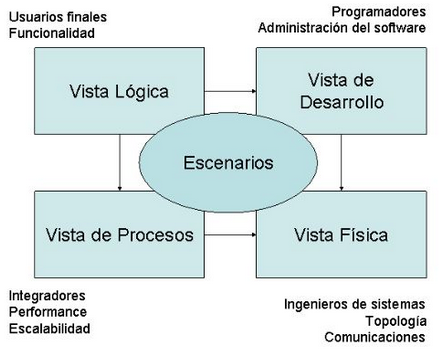
\includegraphics[width=14cm]{modelo4+1vistas.png}
}


\seccion{MODELO 3-DIMENSIONAL SUNTONE.}





\seccion{MODELO VISTA-CONTROLADOR (MVC).}
 
\seccion{PATRONES DE DISEÑO.}




\seccion{PATRONES DE DISEÑO EN JavaEE}






%-------------------------------------------------------------------------------------
\capitulo{MODELO 4+1 VISTAS.}

\seccion{VISTA LÓGICA.}

\seccion{VISTA DE PROCESOS.}

\seccion{VISTA FÍSICA.}

\seccion{VISTA DE DESARROLLO.}

\seccion{ESCENARIOS.}


%-------------------------------------------------------------------------------------
\capitulo{MODELO 3-DIMENSIONAL SUNTONE.} 




%-------------------------------------------------------------------------------------
\capitulo{DEFINICIÓN DE FRAMEWORKS.}

\seccion{DIAGRAMA DE CLASES.}





%-------------------------------------------------------------------------------------
\capitulo{TECNOLOGÍAS A UTILIZAR.}





%-------------------------------------------------------------------------------------
\capitulo{GESTIÓN DEL PROYECTO.}

\seccion{DEFINICIÓN DE ROLES.}

HAY QUE ACTUALIZARLO, SOLO LO DEJÉ PARA MANTENER EL FORMATO.

- \textbf{Elías González Marincovic}: Encargado de la funcionalidad lógica de la aplicación utilizando servicios propios de Java EE, JavaRestfull y encargado de la intercomunicación de los diversos componentes del sistema.\\

- \textbf{Nicolas Rozas Sepúlveda}: Es el especialista en Base de Datos, será el encargado de utilizar las herramientas y administrar la base de datos relacional (distribuir, poblar tablas, etc), utilizando las tecnologías, MySQL y en diseño Sybase PowerDesigner u otras.\\

- \textbf{Daniel Gacitúa Vásquez}: Encargado de la interfaz web que poseerá la aplicación, la cual debe  facilitar las consultas que los usuarios deseen realizar al servidor de aplicaciones mediante una interfaz adecuada, utilizando una presentación correcta para la funcionalidad que se le dará a "BitPhoto". Para esto se utilizará AngularJS, jQuery y HTML5.\\

- \textbf{Gerson Aguirre Pavez}: Encargado de realizar el buscador, parte importante de las vistas que se solicitan, utilizando la herramienta Apache Lucene junto con la aplicación de índices invertidos para la indexación de datos.\\

- \textbf{Max Chacón Villanueva}: Encargado de la aplicación móvil. Estará a cargo de posibilitar el uso de "BitPhoto" en dispositivos Android.\\


Cabe destacar que se asignaron compañeros de apoyo para los diversos roles, quedando la organización de la siguiente manera:

\begin{itemize}
	\item \textbf{Base de Datos}: Encargado Nicolas - Soporte Elías.
	\item \textbf{Aplicación Web}: Encargado Daniel - Soporte Nicolás.
	\item \textbf{Java REST}: Encargado Elías - Soporte Gerson.
	\item \textbf{Aplicación Móvil}: Encargado Max - Soporte Daniel.
	\item \textbf{Buscador}: Encargado Gerson - Soporte Max.
\end{itemize}

También es importante señalar que todos los miembros del Grupo de trabajo estarán encargados de asegurar la calidad del producto (aplicación "BitPhoto"), es decir todos son responsables de la revisión de todos los procesos y tareas que se realicen, además de velar porque se cumplan los resultados que se esperan y que se realice todo de manera correcta.

\newpage

\seccion{DEFINICIÓN DE HERRAMIENTAS.}

A continuación se describe de manera breve y generalizada las tecnologías y herramientas a utilizar para el desarrollo de BitPhoto, para lo cual se han divididoen tres categorías asociadas al sistema a desarrollar, como lo es el Back-End (asociada a la lógica del negocio o lógica de la aplicación), el Front-End (que hace referencia a la parte del sistema que interactúa directamente con el usuario del sistema) y de uso generalizado para el desarrollo del proyecto.  Cabe destacar que las herramientas utilizadas se escogieron con el fin de lograr los requisitos planteados anteriormente.\\

\subseccion{HERRAMIENTAS BACK-END.}

\textbf{Glassfish Server}: Es un servidor de aplicaciones desarrollado por Sun Microsystems, el cual implementa tecnologías definidas para JEE. Es gratuita y de código libre, pero también posee una versión comercial. Posee como servidor base a Sun Java System Application Server de la corporación Oracle. El fin de utilizar Glassfish como servidor de aplicaciones es que permite proporcionar servicios a computadoras clientes, donde los clientes pueden acceder a los datos o conectarse con la parte lógica de la aplicación. Además es compatible con la plataforma JavaEE de esta forma se podrá conectar con JavaEE RESTful.\\

\textbf{MySQL Comunity Edition 5.0+}: Es un sistema que gestiona bases de datos tipo relacional, con capacidad multihilo y multiusuario, desarrollado por Sun Microsystems (MySQL AB), aunque actualmente se desarrolla como software libre, además de poseer una versión comercial. MySQL Comunity Edition es un conjunto de programas que permiten almacenar, modificar y extraer información desde una base de datos, junto con proporcionar herramientas para añadir, borrar, modificar y analizar datos. También cabe destacar que proporciona métodos para mantener la integridad en los datos de la base de datos, controlando el acceso a usuarios, otorgando niveles de permisos para operar sobre la base de datos y recuperar información en caso de ser corrupta mediante una copia de seguridad. Todo lo señalado anteriormente está acompañado y representado mediante una interfaz comoda y facil de utilizar.\\

\textbf{Apache Lucene 4.0+}: Es una API de código abierto, que se agregará como biblioteca al proyecto en Java. Que tiene como fin la búsqueda y recuperacion de informacion, creada por Doug Cutting. Actualmente está apoyado por la fundación de software de Apache y se distribuye bajo la licencia Apache Software License. En este caso se utilizaran sus características de indexado y búsqueda de texto para realizar el buscador de imágenes dentro de BitPhoto. Se basa en el concepto de documentos los cuales poseen determinados campos de texto, permitiendo así trabajar con diferentes formatos de texto.\\

\textbf{Weka 3.5+}: Es una plataforma de software que se caracteriza por el aprendizaje automático y se utiliza frecuentemente en la minería de datos, es una biblioteca escrita en Java y desarrollada por la Universidad de Waikato. Es un software distribuido bajo la licencia GNU GPL. Consiste en una colección de programas con algoritmos de aprendizaje que se encargan de procesar una serie de datos. Estos algoritmos se utilizan para entregar resultados luego de procesar los datos, mediante tareas de clasificación, regresión, asociación, entre otras. Con este conjunto de software se tiene como objetivo crear un analizador de sentimientos, para lo cual se entrenará un modelo con el fin de determinar los sentimientos de los comentarios que realizan los usuarios de BitPhoto, caracterizando estos como positivo, negativo o neutro.\\

\textbf{Netbeans JavaEE 7.0+}: Es un entorno de desarrollo libre, creado principalmente para trabajar con el lenguaje Java. Posee una gran compatibilidad con diferentes tecnologías. Es un producto libre, aunque también existe una versión comercial. Para este proyecto se utilizará para realizar la integración entre las partes de nuestro sistema, conectar la base de datos con la lógica de la aplicación, así también con los módulos respectivos al buscador y clasificador, como también servir la aplicación creada.\\

\subseccion{HERRAMIENTAS FRONT-END.}

\textbf{AngularJS 1.3+}: Es un framework de JavaScript de código abierto, mantenido con el apoyo de google. Tiene como objetivo apoyar la creación de aplicaciones basadas en la capacidad del navegador con un modelo MVC, incluyendo así facilidades para el desarrollo y la prueba del código. El objetivo de utilizar esta herramienta está en desarrollar un esquema de aplicación web basado en rutas, potenciado por el uso de JavaScript y HTML5.\\

\textbf{Bootstrap 3.3+}: Es un framework de diseño web, libre y de código abierto, que contiene una colección de herramientas para la creación de sitios web y aplicaciones web. Contiene código predefinido HTML5 y plantillas CSS, para determinar la forma de los botones, textos, características en la navegación entre otras. Lo utilizaremos también para la creación de la interfaz tanto web de BitPhoto con el fin de agilizar el desarrollo de la interfaz, al mismo tiempo que ésta queda con un diseño adaptativo y homogéneo.\\

\textbf{jQuery 1.x}: Es una biblioteca de JavaScript, creada en un comienzo por John Resing, esta biblioteca permite simplificar la manera de interactuar entre documentos HTML, manejar eventos, desarrollar animaciones, entre otras cosas. Todo esto complementado con la técnica AJAX para la creación de páginas web. Licencia MIT. jQuery otorgará funcionalidades basadas en JavaScript para la creación de BitPhoto, permitiendo lograr grandes resultados en menos tiempo y menos líneas de código.\\

\textbf{HTML5}: Lenguaje de marcado para la creacion de paginas web. Es un lenguaje estándar que sirve de referencia para la elaboración de sitios web. Para este caso permitirá definir una estructura básica para la interfaz de la aplicación y un código para la definición de contenido web como lo son textos, imágenes, videos, entre otros. En estwe caso se utilizará el último estándar de este lenguaje, que es HTML5.\\

\textbf{CSS3}: Hojas de estilo en cascada o CSS, lenguaje utilizado para la definición de plantillas web, para formatos HTML o XML. Permite estandarizar el diseño en la creación de aplicaciones web. La utilización de CSS 3, última versión de CSS, permitirá estilizar uniformemente la apariencia de los elementos de la aplicación.\\

\textbf{JavaScript 1.8+}: Lenguaje de programación interpretado, quiere decir que se ejecuta del lado del navegador. Se caracteriza por ser orientado a objetos, basado en prototipos y se imperativo. Para este proyecto nos permitirá mejorar la interfaz de usuario y generar paginas web dinamicas.\\

\textbf{Android SDK 19}: Sistema Operativo basado en el kernel de Linux, actualmente desarrollado por Google, y utilizado en dispositivos móviles de manera masiva. Para este caso se desarrollará una aplicación compatible con este sistema operativo para que los usuarios de BitPhoto puedan hacer uso de éste a través de sus dispositivos móviles. Para esto se utilizará el SDK versión 19 para compatibilizar la aplicación con todos los dispositivos Android de versión 4.0 en adelante.\\

\subseccion{HERRAMIENTAS USO GENERAL.}

\textbf{Git}: Es un software que permite controlar las versiones, fue diseñado por Linus Torvalds, con el fin de controlar de manera eficiente y confiable las versiones de archivos de código fuente. El repositorio remoto a utilizar será proporcionado por GitHub el cual entrega espacio para desarrollar el proyecto, y conectar éste con los miembros del equipo de trabajo.\\


\textbf{Gradle}: Es una herramienta de automatización de proyecto, se basa en los principios de Apache Ant y Maven. Permite controlar y configurar el proyecto. Utiliza un grafo dirigido para determinar el orden de las tareas que se pueden ejecutar. Para esta entrega se utilizará Gradle para compilar, desplegar, testear y controlar las diferentes dependencias del proyecto.\\

\textbf{JUnit}: Es un conjunto de bibliotecas creadas para la programación, con el fin de realizar pruebas unitarias sobre diversos componentes de la aplicación, en especial las realizadas en Java. Nos permitirá ejecutar las clases creadas en Java, de manera controlada para evaluar el funcionamiento de los métodos implementados. Entonces en función de algún valor de entrada para la prueba se evalúa el valor retornado. si es el esperado o no. También se utlizará para controlar las pruebas de regresión, para que cuando se modifique el código se pueda corroborar si el nuevo código cumple con los requerimientos anteriores.\\

\newpage

\seccion{ORGANIZACIÓN DE REPOSITORIOS GIT.}
    
Para optimizar la creación de código, favorecer la correcta colaboración entre los integrantes y tener un versionamiento ordenado del código, se decide emplear a git como sistema de control de versiones, y usar GitHub como servidor remoto de git.\\

Cada miembro del grupo utiliza una cuenta de GitHub:

\begin{itemize}
	\item \textbf{Gerson Aguirre}: \textsl{https://github.com/GersonAguirre}
	\item \textbf{Max Chacón}: \textsl{https://github.com/nanochacon}
	\item \textbf{Daniel Gacitúa}: \textsl{https://github.com/GaciX}
	\item \textbf{Elías González}: \textsl{https://github.com/Elitos}
	\item \textbf{Nicolás Rozas}: \textsl{https://github.com/NicoRozas}
\end{itemize}

Se ha creado la organización “tbd2015” que aloja todos los repositorios del proyecto: \textsl{https://github.com/tbd2015}.\\

Dentro de la organización, se han creado diferentes repositorios para cada módulo del proyecto:

\begin{itemize}
	\item \textbf{InformesTBD}: Contiene los informes y presentaciones del proyecto. 
	\item \textbf{Prototipo}: Contiene el prototipo gráfico de la Aplicación Web.
	\item \textbf{BitPhoto}: Contiene el módulo principal del proyecto (en JavaEE).
	\item \textbf{BitPhoto-Mobile}: Contiene la aplicación para Android del proyecto.
	\item \textbf{BitPhoto-Search}: Contiene el motor de búsqueda (potenciado por Apache Lucene).
	\item \textbf{BitPhoto-Miner}: Contiene el módulo de análisis de sentimientos (potenciado por Weka).
\end{itemize}

Cada miembro del grupo tendrá acceso a todos los repositorios para fomentar la colaboración. Cabe destacar que con un sistema modular de repositorios dentro de la organización ordena de mejor manera los aportes de cada miembro y ayuda a evitar el entorpecimiento al hacer commits de forma concurrente.

\newpage

\seccion{COMUNICACIÓN, AVANCES Y BURNDOWN.}

En la primera reunión realizada planificamos el Sprint, se determinó que el primer Sprint duraría hasta el 17 de Abril del 2015. Además se acordó las horas de trabajo diarias que se podían dedicar a la realización del proyecto, se estimó que cada integrante del grupo podría dedicar a lo máximo 1.5 hrs al dia para el proyecto. Luego se definieron las tareas para que estas se pudieran realizar en un tiempo cercano al de trabajo diario estimado, luego se estimó el tiempo que se demoraría cada tarea en estar realizada. 

Para la realización de la primera entrega el grupo optó por varios canales de comunicación para manejar las relaciones entre los participantes, por lo tanto se determinaron distintas tecnologías para objetivos específicos, los canales usados para comunicarse entre el grupo fueron los siguientes:

\begin{itemize}
	\item Se creó un grupo en WhatsApp, con el fin de conversar inmediatamente y de forma rápida temas relacionados con el proyecto, principalmente se utilizó para dudas cortas y compartir pequeñas opiniones del proyecto. 
	\item Se creó un grupo en Facebook, para registrar minutas, información relevante y noticias que afecten a todos los integrantes del grupo.
	\item Se creo una carpeta en google drive, para con el fin de compartir documento referentes al informe, presentaciones, etc.  
	\item Se utilizó la aplicación Trello para organizar las partes que se debían realizar en la entrega, además esta aplicación permite organizar las partes del proyecto definiendo las tareas personalmente y los tiempos con los que fueron realizadas cada una de estas.
	\item Para controlar las versiones del informe y los prototipo de las vistas se utilizó la herramienta Git que permite controlar las versiones de estas dos partes del proyecto, esta tecnología se utiliza para archivos de texto plano y para controlar las modificaciones que se le pueden realizar a estos.
\end{itemize}

\newpage

A continuación se presentan las tareas definidas y los tiempos estimados.

\figura{Tareas 1-15}{
	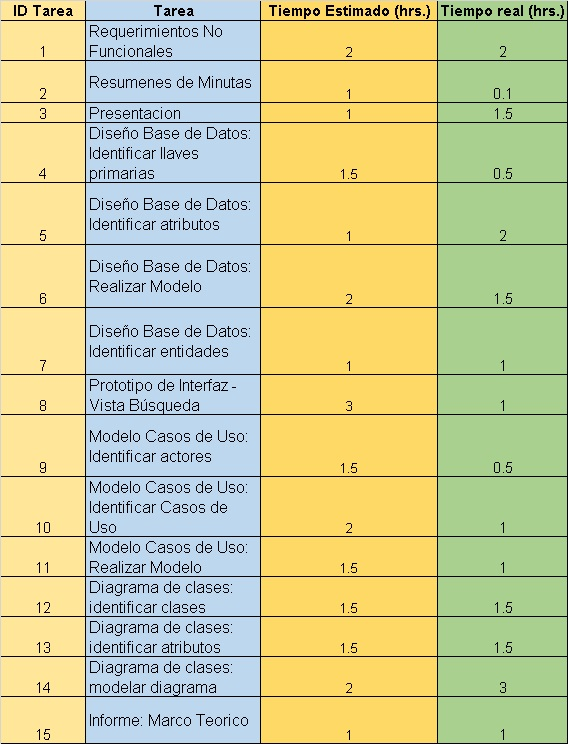
\includegraphics[width=14cm]{burndown/Tareas1.jpg}
}

\figura{Tareas 16-32}{
	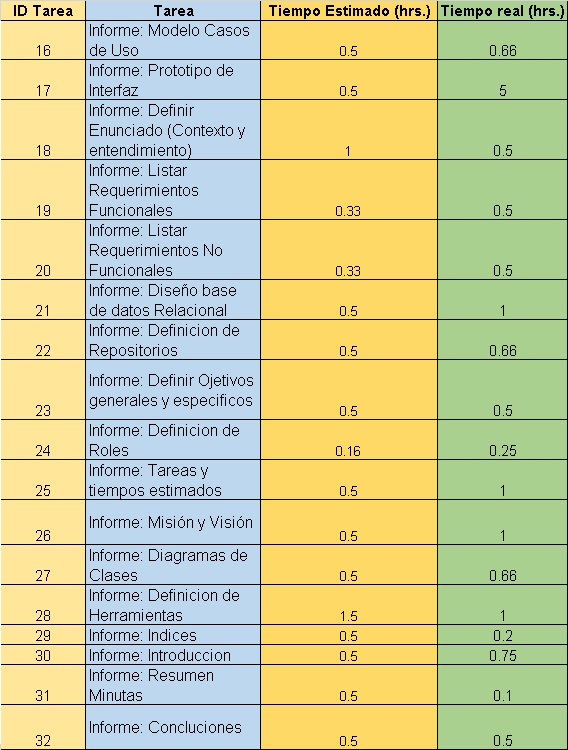
\includegraphics[width=14cm]{burndown/Tareas2.jpg}
}

\figura{Tareas 33-49}{
	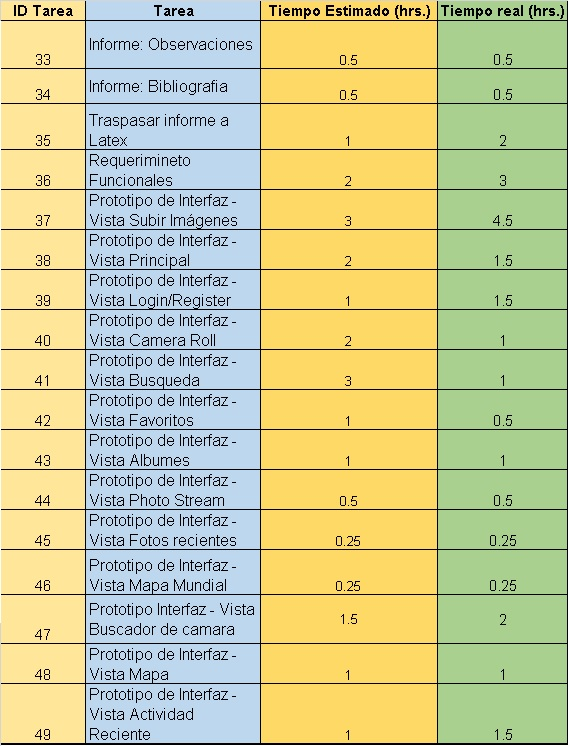
\includegraphics[width=14cm]{burndown/Tareas3.jpg}
}

Ahora la cantidad de horas de trabajos estimadas son 54.32 hrs, Las horas de trabajo real fueron 56.38, notar que las horas reales trabajadas superaron las horas estimadas en 2.06 hrs aprox, esto quiere decir que las tareas se estimaron correctamente en su mayoría, ya que este margen de error fue relativamente bajo. Tiempo promedio por tarea fue de 1.11 hrs. Otros datos que se obtiene al analizar lo anterior son:

\begin{itemize}
	\item Estimación Trabajo Diario Grupo: 7.5 
	\item Horas Disponibles en Sprint por cada integrante: 37.5 
	\item Horas Disponibles en Sprint del Grupo: 187.5 
	\item Trabajo por dia promedio ideal 2.59 
\end{itemize}

Cabe señalar que si se trabajara de manera ideal, sobraría  tiempo equivalente a 187.5 hrs - 54.32 hrs = 133.18 hrs. Al pasar una semana se creyó que era necesario definir los roles de cada miembro del grupo para comenzar a trabajar o informarse desde ahora sobre el área en particular designada.

A continuación se presentan los gráficos BurnDown y BurnUp con el fin de señalar la forma en que se trabajó a lo largo del Sprint:

\figura{Gráfico de Burndown/Burnup}{
	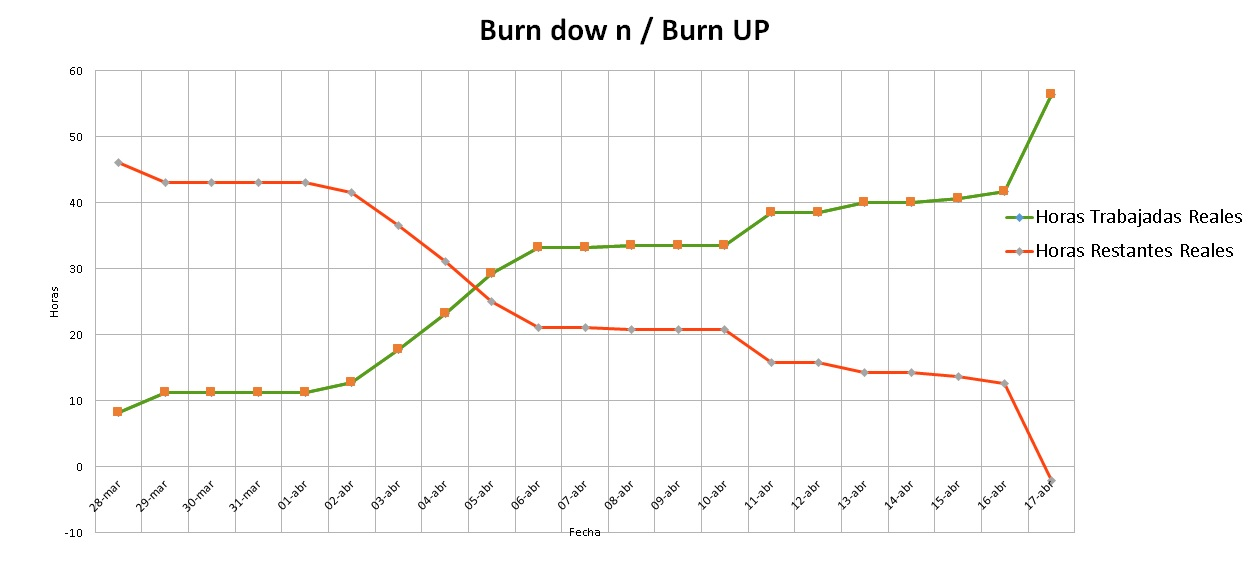
\includegraphics[width=14cm]{burndown/burndown2.jpg}
}

Como se aprecia en la imagen, se observa que en determinados periodos se trabajo una mayor cantidad, si bien alcanzamos a realizar la mitad del trabajo estimado a la fecha 5 de Abril, luego se disminuyó el trabajo realizado por dia a una frecuencia menor, en los últimos días se aumentó la frecuencia de trabajo para el los días antes de la entrega del informe. Otra cosa que se aprecia es que desde el primer dia en el que se definió el SPRINT se comenzó a trabajar por eso la grafica no comienza desde cero.



%-------------------------------------------------------------------------------------
\capitulo{OBSERVACIONES.}

Se añaden las observaciones realizadas al trabajo durante la 1º Presentación del Proyecto:

\tabla{Observación OBS1}{
	\begin{tabular}[c]{|p{4cm}|p{11cm}|}
		\hline
		Número Observación & OBS1\\ \hline
		Detalle Observación & El RF41 es un requisito funcional del browser no de la aplicacion.\\ \hline
		Acción a Realizar & Se elimina el RF41 (El usuario puede mantener sus sesión iniciada mediante la opción “Recordar sesión”).\\ \hline
		Justificación & Este requisito es del navegador web, no de la aplicación en si.\\ \hline
		Página del Informe & 22\\ \hline
	\end{tabular}
}

\tabla{Observación OBS2}{
	\begin{tabular}[c]{|p{4cm}|p{11cm}|}
		\hline
		Número Observación & OBS2\\ \hline
		Detalle Observación & El RNF4 tiene que especificar el estandar de los datos geo-espaciales.\\ \hline
		Acción a Realizar & Redactar nuevamente en el requisito no funcional numero 4.\\ \hline
		Justificación & En el requisito se debe especificar el formato estandar que utilizan los datos geo-espaciales.\\ \hline
		Página del Informe & 23\\ \hline
	\end{tabular}
}

\tabla{Observación OBS3}{
	\begin{tabular}[c]{|p{4cm}|p{11cm}|}
		\hline
		Número Observación & OBS3\\ \hline
		Detalle Observación & Explicacion de los canales de comunicacion.\\ \hline
		Acción a Realizar & Redactar un texto que muestre los canales de comunicacion utilizados en la realizacion de la entrega.\\ \hline
		Justificación & Por proósitos de documetnación, en el informe se deben detallar los canales que utilizaron los participantes.\\ \hline
		Página del Informe & 52\\ \hline
	\end{tabular}
}

\newpage

\tabla{Observación OBS4}{
	\begin{tabular}[c]{|p{4cm}|p{11cm}|}
		\hline
		Número Observación & OBS4\\ \hline
		Detalle Observación & En el grafico de Burndown mostrar solo curvas reales.\\ \hline
		Acción a Realizar & Cambiar el grafico de burdown con otro con solo las curvas reales del trabajo.\\ \hline
		Justificación & Muchas lineas confunden al que observa el grafico, este deberia ser mas simple y solo mostrar las curvas reales.\\ \hline
		Página del Informe & 56\\ \hline
	\end{tabular}
}

%-------------------------------------------------------------------------------------
\capitulonn{CONCLUSIONES.}

Luego de finalizar la primera entrega del proyecto correspondiente a la ingeniería de requerimientos, se ha concluido en dos perspectivas que se estiman adecuadas a la hora de realizar futuros trabajos, perspectiva a nivel de la ingeniería de requerimientos y la perspectiva de trabajo en equipo.

Con respecto a la ingeniería de requerimientos y ciertos aspectos utilizados a la hora de realizar la entrega, se puede decir que las herramientas utilizadas y mencionadas con anterioridad en el informe, han facilitado muchos aspectos, agregando además que han ampliado la perspectiva del proyecto, logrando así entender en profundidad cómo funciona el sistema a crear, cuales son estas funcionalidades y cómo se pueden crear a futuro.

Es por esto que se puede decir que esta etapa en la ingeniería de software es fundamental a la hora de iniciar el proyecto.

En la otra perspectiva a nivel del trabajo en equipo, se puede concluir que se ha logrado una gran comunicación entre cada uno de los integrantes del grupo y una buena organización debido a esto mismo, en conjunto con las herramientas de carácter social se ha logrado un gran avance en relación al trabajo en equipo.

Finalmente como conclusión general se puede decir que se ha trabajado de manera íntegra cumpliendo a cabalidad los objetivos específicos tanto como generales que se han planteado.


%-------------------------------------------------------------------------------------

\capitulonn{BIBLIOGRAFÍA.}

\begin{itemize}
	\item Glassfish: https://glassfish.java.net/es/
	\item MySQL: http://www.mysql.com/
	\item Weka: http://www.cs.waikato.ac.nz/ml/weka/
	\item Bibliografia: https://lucene.apache.org/
	\item Netbeans: https://netbeans.org/
	\item AngularJS : https://angularjs.org/
	\item Bootstrap: http://getbootstrap.com/
	\item JQuery: https://jquery.com/
	\item CSS3: http://www.css3.info/
	\item HTML5: http://www.w3schools.com/html/html5\_intro.asp
	\item JavaScript: http://www.w3schools.com/js/
	\item Android: https://www.android.com/
	\item Git: http://git-scm.com/
	\item Gradle: https://gradle.org/
	\item JUnit : http://junit.org/
	\item Diagrama de clases: http://users.dcc.uchile.cl/~psalinas/uml/modelo.html
	\item Mision y Vision: http://es.slideshare.net/ponceguillermo71/concepto-de-mision-y-vision
\end{itemize}

\end{document}
